% 1977 年黑龙江卷附加题第 9 题：曲柄连杆机构，圆心 O、曲柄 OA（半径 R）、
% 连杆 AP（l）、曲柄转角 α 标在 O 处，P 在 x 轴上（按源卷布局）
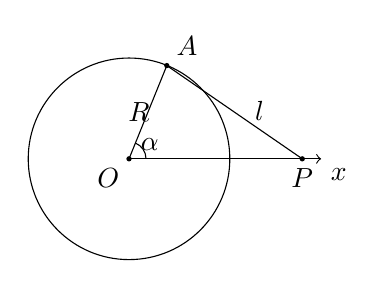
\begin{tikzpicture}[scale=0.8]
  \draw (0,0) circle (1.6);
  \coordinate (O) at (0,0);
  \coordinate (A) at (0.60,1.48);
  \coordinate (P) at (2.75,0);
  \draw[->] (0,0) -- (3.05,0) node[below right] {$x$};
  \draw (O) -- (A);
  \draw (A) -- (P);
  \draw (0.27,0) arc (0:68:0.27);
  \fill (O) circle (1.2pt) node[below left] {$O$};
  \fill (A) circle (1.2pt) node[above right] {$A$};
  \fill (P) circle (1.2pt) node[below] {$P$};
  \node at (0.16,0.75) {$R$};
  \node at (2.07,0.76) {$l$};
  \node at (0.33,0.22) {$\alpha$};
\end{tikzpicture}
